\documentclass[10pt,a4paper]{article}
\usepackage[utf8]{inputenc}
\usepackage[english]{babel}
\usepackage{amsmath}
\usepackage{amsfonts}
\usepackage{amssymb}
\usepackage{graphicx}

\title{COS 301 Software Documentation}
\author{Melany Barnes 12030466 \\
		Dieter Doman 11002566 \\
		Johan Esterhuyse 10043285 \\
		Rudiger Roach 11004322 }
\date{}
\begin{document}
\maketitle
\begin{center}
Version 1.0 \\
GitHub link: https://github.com/RudigerRoach/301\textunderscore main\textunderscore emma.git \\
\vspace*{5\baselineskip}
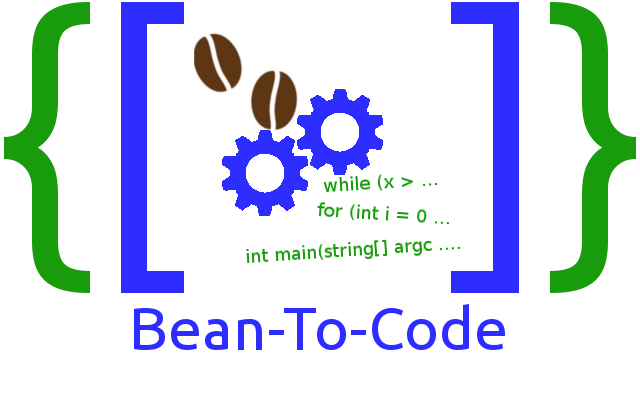
\includegraphics[scale=0.35]{Pictures/Logo.png}
\end{center}
\pagebreak
\tableofcontents
\pagebreak
\section{Vision and Scope}

\subsection{Vision}
Our client creates software for camera club event management. A big part of an event comprises of an image judging process. Currently the process is completed by using Infra-red remotes and receivers but this configuration is limited in terms of usability and the amount of judges that can judge concurrently.\\\\
The proposed solution will replace the hardware remote with a software application to run on a mobile device. The mobile application should alleviate all of the issues caused by the current setup and should be developed with a server component that plugs into the existing EMMA system.  

\subsection{Scope}
Create a software solution that:
\begin{itemize}
\item Runs on IOS and Android mobile devices.
\item Allows as many as 20+ judges on the night.
\item Allows judges to register against the event (in order to score) by capturing an email address.
\item Remembers the scoring device for future meetings such that registration is not required again.
\item Caters for realtime scoring.
\item Can display a thumbnail image of that currently being judged.
\item Caters for simple score entry bound within a variable range.
\item Reports meaningful error messages, in a clear way.
\item Allows for quick correction and re-capture.
\item Can notify a judge of outstanding scores.
\end{itemize}

\begin{figure}  
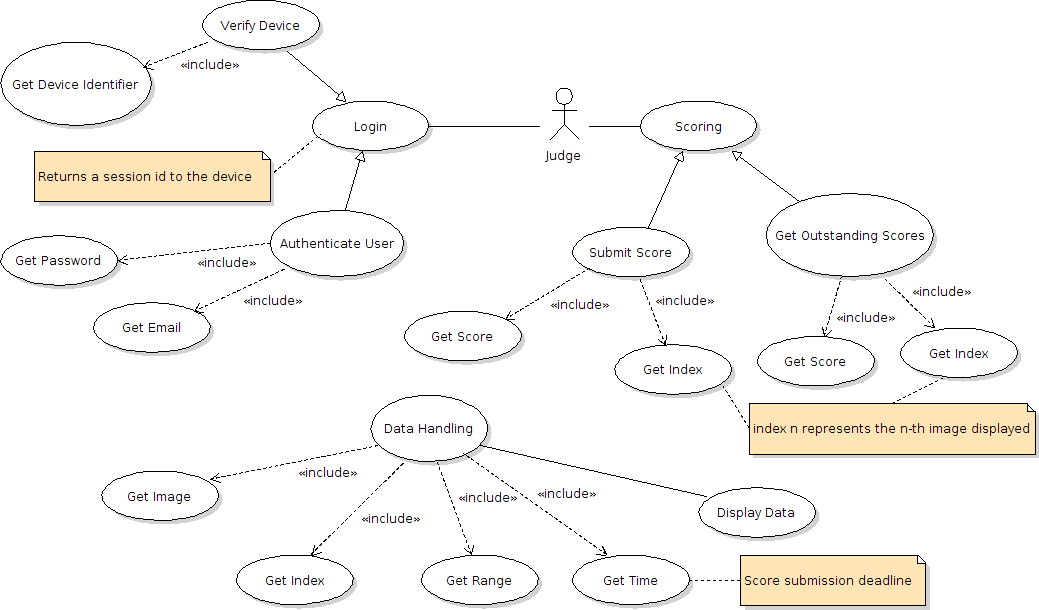
\includegraphics[scale=0.4]{Pictures/High-level-use-case.png}
\caption[Long caption]{High Level Use Case Diagram}
\label{pic-a}
\end{figure}
\pagebreak
\section{Architecture requirements}
\subsection{Architecture requirements}
\subsubsection{Architectural scope}
\begin{itemize}
\item Provide an infrastructure for a judge to rate photos on a mobile device.
\item Provide a database to link a judge's phone id to his email address.
\end{itemize}
\subsubsection{Quality requirements}
\begin{itemize}
\item Security \\
The systems functionality should be only available to users who can be authenticated through the EMMA system. New users have to create an account before being granted access to the application.
\item Usability \\
99 \% of users should be able to use the system with little to no prior training.
\item Testability \\
All services offered must be accompanied by unit tests. The tests should ensure that all pre-conditions are met before the service is delivered and that all post-conditions are met after the service has been delivered.
\item Performance requirements \\
 All operations on application should respond within less than 1 second.
\item Scalability \\
The deployed system must be able to operate effectively under the load of 50 concurrent users.
\item Installability \\
It should be easy to install the server side component and the effort to get it running each club night should be minimal. The application should also be easy to download and install.
\end{itemize}
\subsubsection{Integration and access channel requirements}
\begin{itemize}
\item Integration requirement \\
The production version of this application will need to integrate with EMMA. EMMA is Java a based application.
\item Access channels \\
The mobile application will have to go through a web-service which will be the public interface for the server-side component. 
\end{itemize}
\subsubsection{Architectural constraints}
\begin{itemize}
\item The mobile application should run on Android and iOS operating systems.
\item The PC's that will be running the server side of the application and EMMA component will generally not be the latest technology(limited memory and processing power).
\item There will be limited to no internet connection.
\item The communication between the mobile device and server PC will be done over a wifi network.
\item The server side component of this project should be able to run on Windows and OS X operating systems.
\end{itemize}
\subsection{Use of reference architectures and frameworks}
\begin{itemize}
\item JIRA Framework for the SCRUM agile method.
\item Appcelerator Titanium framework which is an open-source software development kit for cross-platform mobile development.
\item Jetty for hosting server.
\item Drillbit framework to run javascript unit  testing in the Titanium framework.
\item JUnit for java unit testing framework.
\end{itemize}
\subsection{Technologies and languages}
\begin{itemize}
\item Java
\item JavaScript
\item XML
\item MySQL Database
\end{itemize}
\section{Functional requirements and application design}
\subsection{Introduction}
This section discusses the functional requirements for the mobile judging system.
\subsection{Required Functionality}
\subsubsection{Login}
To login for the first time a user will have to enter his email address. The email provided will be authenticated by EMMA. If login fails the user will be informed that he is not registered to be a judge for the current session. If login is successful the device's unique identifier will be sent to the server to be stored in the database so that the device can be remembered on the system. This will allow for auto login - if a user attends a session where he is able to judge his phone will automatically be logged into the system. The user will then be able to use the rest of the system.

\begin{center}
\advance\leftskip-1.3cm
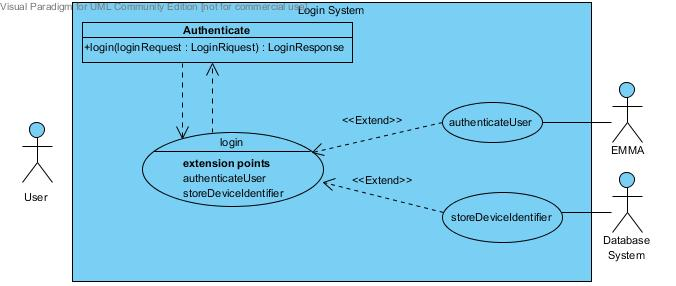
\includegraphics[width=160mm]{Pictures/Login.jpg} 
Login Use Case Diagram 
\end{center}

\subsubsection{Judging Session}
When the server is started, it will request that the session's photos as well as all the competition constraints be sent to it. The constraints will contain the type of session (Open event, Closed event, Yes/No, Winner), the range for a valid score and if comments are enabled.

\begin{center}
\advance\leftskip-1.3cm
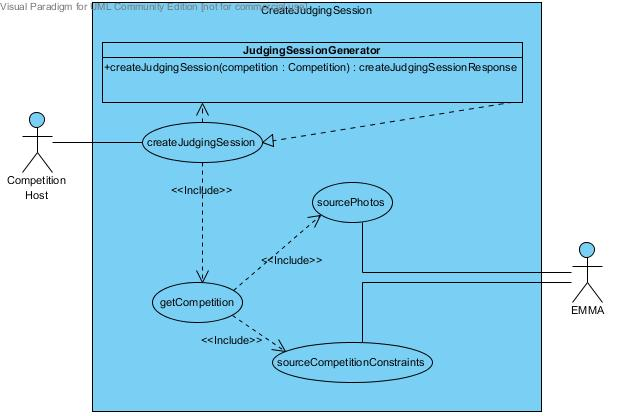
\includegraphics[width=130mm]{Pictures/CreateJudgingSession.jpg} 
Create Judging Session Use Case Diagram 
\end{center}

\subsection{Use case prioritization}
Critical Use Cases are the main cases that the system is made up of namely: Login, Create Judging Session. Without these cases the system will have limited to no functionality which will lead to a system that is not required by anyone.
\\ \\
Important Use Cases are the cases that improves the critical use cases and introduces a wider variety of functionality. These cases are Auto Login.

%Nice-To-Have Use Cases make the system more user friendly and provides a better user experience. This case is: 

\subsection{Use case/Services contracts}
\begin{center}
\advance\leftskip-1.3cm
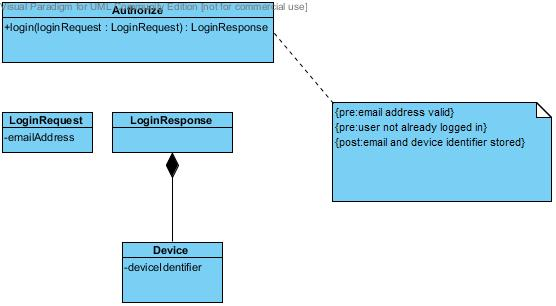
\includegraphics[width=160mm]{Pictures/servicesContractLogin.jpg} 
Services contract for Login
\end{center}

\begin{center}
\advance\leftskip-1.3cm
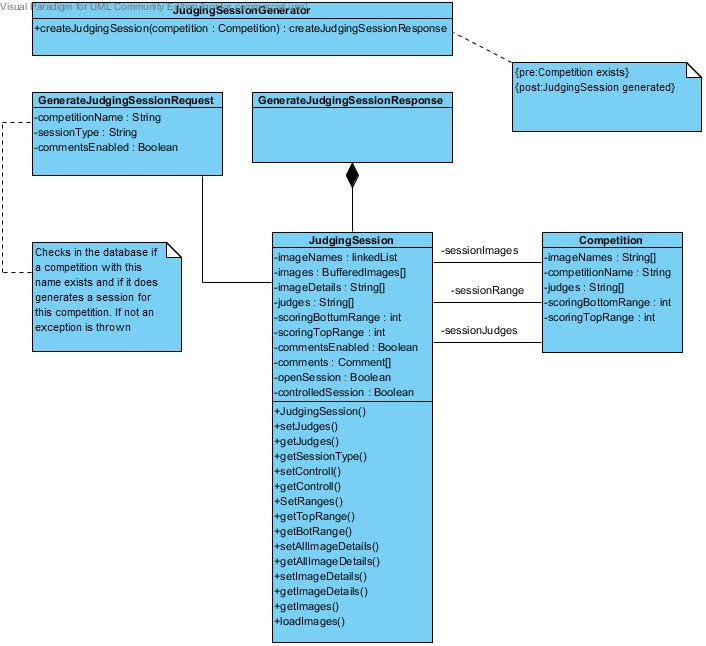
\includegraphics[width=160mm]{Pictures/servicesContractCreateJudgingSession.jpg} 
Services contract for Create Judging Session
\end{center}
\subsection{Process specifications}
\begin{center}
\advance\leftskip-1.3cm
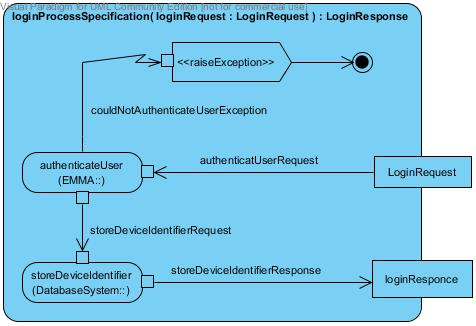
\includegraphics[width=160mm]{Pictures/LoginActivityDiagram.jpg} 
Login Activity Diagram 
\end{center}
\begin{center}
\advance\leftskip-1.3cm
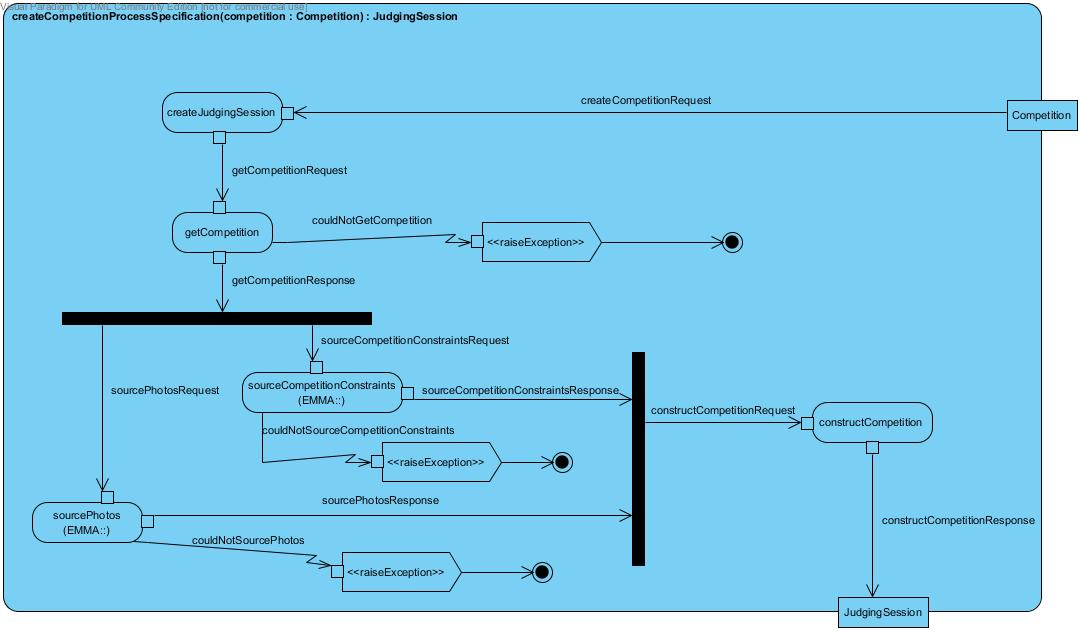
\includegraphics[width=160mm]{Pictures/createJudgingSessionActivityDiagram.jpg} 
Create Judging Session Activity Diagram 
\end{center}
\subsection{Domain objects}
\section{Glossary}
EMMA - Entry and Member Management Application\\
His - Refers to his/her\\
He - Refers to he/she
\end{document}